\clearpage
\phantomsection

\setcounter{chapter}{2}
\chapter[CÀI ĐẶT VÀ THỰC NGHIỆM]{CÀI ĐẶT VÀ THỰC NGHIỆM}

Chương này mô tả cách hiện thực hệ thống đã thiết kế ở Chương~2, tập trung vào những quyết định kỹ thuật ảnh hưởng đến kết quả thực nghiệm. Trọng tâm là ma trận ablation 9 run để cô lập tác động từng kỹ thuật, và hai run mở rộng run59/run62 để kiểm tra observation bottleneck. Cấu trúc: pipeline PCGNN → CombatAgent → cấu hình huấn luyện → thiết kế ablation.

\section{Môi trường phát triển}

Môi trường game được xây dựng bằng Unity 6 và TopDown Engine. Phần học tăng cường dùng Unity ML-Agents để kết nối cảnh chơi Unity với trainer Python. Các thí nghiệm chính được chạy bằng bản build standalone ở chế độ không đồ họa, với nhiều môi trường song song để tăng tốc độ thu thập mẫu.

\begin{table}[H]
    \centering
    \small
    \caption{Môi trường triển khai và huấn luyện}
    \label{tab:development_environment}
    \begin{tabular}{|p{5cm}|p{8cm}|}
        \hline
        \textbf{Thành phần} & \textbf{Cấu hình sử dụng} \\
        \hline
        Game engine & Unity Editor 6000.1.3f1. \\
        \hline
        Gameplay framework & TopDown Engine v4.4, môi trường demo Koala2D được mở rộng cho bài toán RL. \\
        \hline
        Unity package & com.unity.ml-agents phiên bản 4.0.3. \\
        \hline
        Trainer & Unity ML-Agents Python trainer, thuật toán PPO, log qua TensorBoard. \\
        \hline
        Phần cứng & CPU 16 luồng, RAM 16GB, NVIDIA GeForce RTX 3050 6GB. \\
        \hline
        Chế độ chạy & Build standalone, --no-graphics, time-scale=20, thường dùng 8 môi trường song song; một số run dùng 16 môi trường. \\
        \hline
    \end{tabular}
\end{table}

Việc dùng build standalone thay vì chạy trực tiếp trong Editor giúp giảm nhiễu do giao diện và ổn định tốc độ mô phỏng. Với cấu hình 3 triệu bước, thời gian huấn luyện một run đầy đủ thường nằm ở thang nhiều giờ, trong đó phần tốn thời gian nhất là mô phỏng Unity và đồng bộ nhiều môi trường, không phải forward pass của mạng MLP.

\section{Hiện thực pipeline sinh bản đồ bằng PCGNN}

Pipeline bản đồ được tách thành hai giai đoạn. Giai đoạn ngoại tuyến chạy trong môi trường Python của PCGNN để sinh, đánh giá và chia bản đồ theo độ khó. Giai đoạn trong Unity chạy thông qua TilemapGenerator để nạp bản đồ đã chọn vào episode huấn luyện. Cách tách này là cải tiến quan trọng so với phương án gọi generator trực tiếp từ Unity: quá trình huấn luyện ổn định hơn, bản đồ có thể được kiểm tra trước, và người thiết kế vẫn có quyền chọn những bản đồ phù hợp nhất trước khi đưa vào tập huấn luyện chính.

Ở giai đoạn PCGNN, đề tài sử dụng genome đã huấn luyện \emph{inctyseed0.pkl} và logic sinh từ notebook \emph{improve-v2.ipynb}. Mỗi ô bản đồ được sinh theo thứ tự quét từ trái sang phải, từ trên xuống dưới; mạng nhận ngữ cảnh cục bộ $3 \times 3$ xung quanh ô hiện tại cùng bốn đầu vào ngẫu nhiên, sau đó quyết định ô đó là tường hay sàn. Kết quả sau đó được bộ chuyển đổi chuyển sang text map của game.

Để người đọc có trực giác về sự khác nhau giữa thiết lập PCGNN tham chiếu và biến thể dùng trong khóa luận, Hình~\ref{fig:pcgnn_baseline_vs_improved} đặt cạnh nhau các mẫu bản đồ sinh từ hai genome đại diện. Phía baseline dùng checkpoint \emph{neat\_winner\_seed0.pkl} của notebook \emph{BaseLine.ipynb}, tương ứng với kiến trúc NEAT feed-forward trong nghiên cứu PCGNN. Phía cải tiến dùng checkpoint \emph{inctyseed0.pkl}, tương ứng với generator recurrent được dùng để tạo tập bản đồ chính cho Unity. Hai bên cùng giữ quy ước P/E, nhưng bản cải tiến tạo ra nhiều hành lang dài và cấu trúc định hướng hơn, phù hợp với mục tiêu tuyển chọn bản đồ cho curriculum.

\begin{figure}[H]
    \centering
    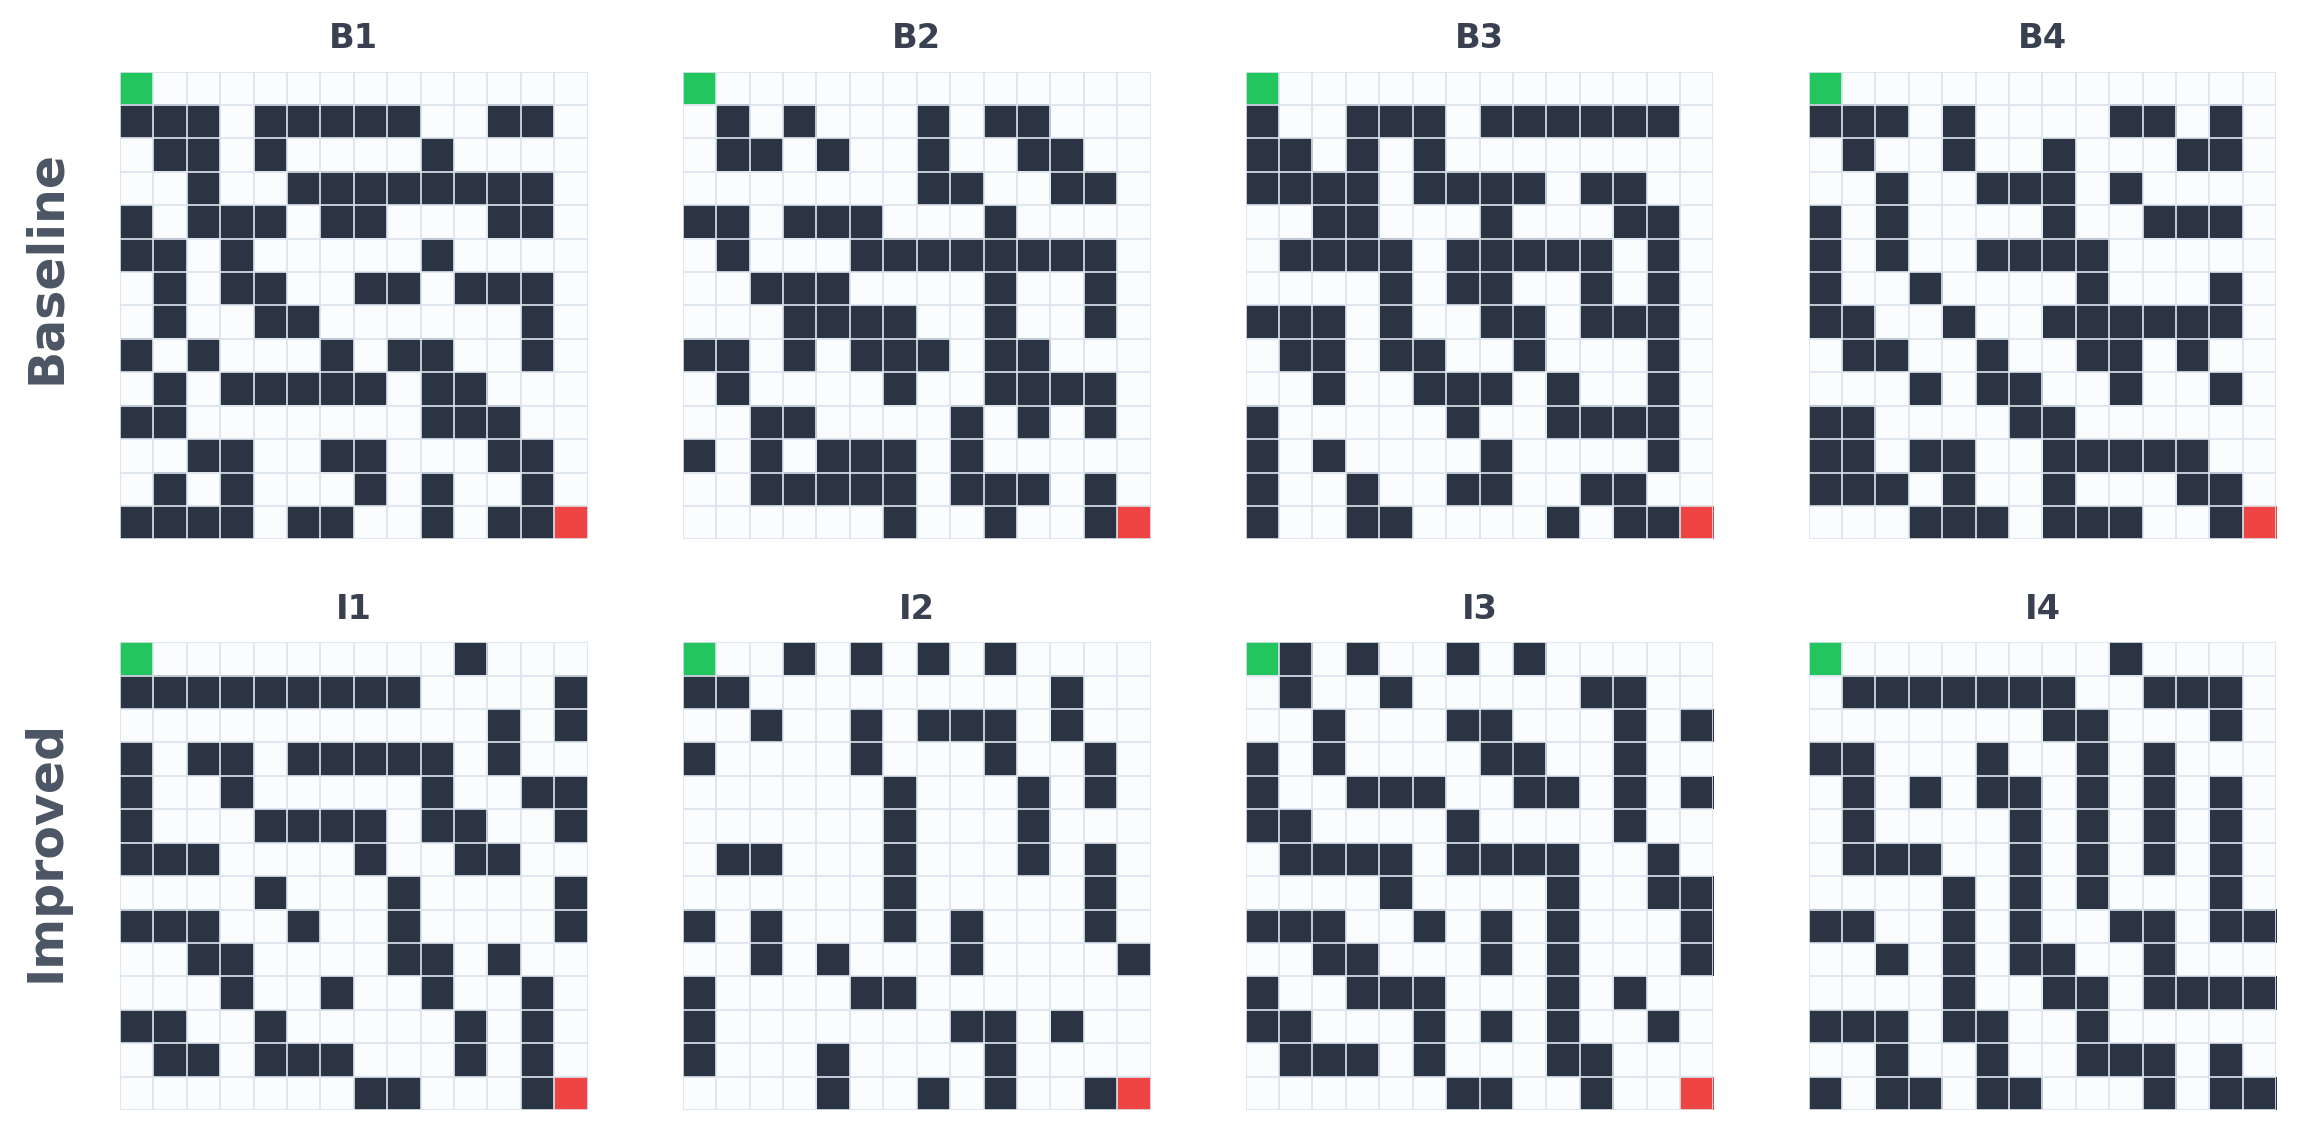
\includegraphics[width=\textwidth]{figures/pcgnn/map_baseline_vs_improved.png}
    \caption{So sánh mẫu bản đồ baseline PCGNN và mẫu bản đồ cải tiến dùng trong khóa luận}
    \label{fig:pcgnn_baseline_vs_improved}
\end{figure}

Hình~\ref{fig:pcgnn_baseline_vs_improved} đóng vai trò so sánh tổng quan giữa hai hướng sinh bản đồ. Các hình ở phần sau sẽ làm rõ hơn hai ý cụ thể: baseline PCGNN thường tạo các đường đi kiểu mê cung nối hai góc, còn bản cải tiến của khóa luận sau bước bộ chuyển đổi sẽ được đánh giá thêm bằng BFS, khả năng đi tới và điểm độ khó trước khi đưa vào các nhóm Easy, Medium và Hard.

\subsection{Điều chỉnh PCGNN cho bài toán Roguelike}

Nghiên cứu của Beukman và cộng sự dùng PCGNN như một bộ sinh level độc lập và đánh giá chất lượng bằng các chỉ số như leniency, A* difficulty, compression distance và A* diversity~\cite{Beukman2022}. Trong khóa luận này, PCGNN được giữ lại ở vai trò bộ sinh ma trận nền, nhưng được mở rộng thành một pipeline phục vụ trực tiếp cho huấn luyện tác nhân trong Unity. Các điểm điều chỉnh chính được tóm tắt trong Bảng~\ref{tab:pcgnn_improvements}.

\begin{table}[H]
    \centering
    \small
    \caption{Các điều chỉnh PCGNN trong khóa luận}
    \label{tab:pcgnn_improvements}
    \begin{tabular}{p{4.0cm} p{5.0cm} p{5.0cm}}
        \toprule
        \textbf{Thành phần} & \textbf{Thiết lập PCGNN tham chiếu} & \textbf{Điều chỉnh trong khóa luận} \\
        \midrule
        Vai trò của generator & Sinh level để đánh giá chất lượng và độ đa dạng của nội dung. & Sinh tập bản đồ ngoại tuyến để đưa vào curriculum learning trong Unity. \\
        Biểu diễn đầu ra & Ma trận tile của miền Maze/Mario trong thiết lập tham chiếu. & Chuyển sang text map của game với ký hiệu \#, ., P, E. \\
        Xử lý vị trí người chơi và kẻ địch & Phụ thuộc vào biểu diễn của từng miền sinh bản đồ. & Adapter đặt P/E trên cùng thành phần liên thông lớn nhất và chọn hai vị trí cách xa nhau. \\
        Kiểm tra hợp lệ & Đánh giá bằng các chỉ số ngoại tuyến. & BFS xác nhận đường đi từ P tới E; TilemapGenerator kiểm tra lại vùng đi được khi nạp bản đồ. \\
        Chỉ số bổ sung & Các chỉ số PCGNN gồm leniency, A* difficulty, compression distance và A* diversity. & Bổ sung các chỉ số reachable\_ratio, dead\_end\_ratio và difficulty\_score để phục vụ chọn bản đồ cho curriculum. \\
        Tổ chức dữ liệu & Không gắn với lesson của môi trường Unity. & Chia bản đồ thành Easy/Medium/Hard theo percentile để điều khiển độ khó huấn luyện. \\
        Tích hợp lúc chạy & Không hướng tới gọi trực tiếp trong Unity. & Tách generator ngoại tuyến và TilemapGenerator trong Unity để giảm độ trễ, tăng khả năng tái lập và cho phép kiểm tra bản đồ trước. \\
        \bottomrule
    \end{tabular}
\end{table}

Do đó, phần ``cải tiến'' trong khóa luận không nằm ở việc thay đổi hoàn toàn thuật toán NEAT của PCGNN, mà nằm ở lớp hậu xử lý, kiểm định, đo khả năng đi tới và tích hợp bản đồ vào curriculum. Cách làm này phù hợp với mục tiêu của đề tài: tạo một tập bản đồ sinh theo thủ tục đủ đa dạng nhưng vẫn kiểm soát được tính hợp lệ trước khi dùng để huấn luyện CombatAgent.

\subsection{Adapter và kiểm tra hợp lệ}

Adapter thực hiện ba việc: chuyển ma trận tile của PCGNN sang ký tự \# và dấu chấm (.); tìm thành phần liên thông lớn nhất của vùng sàn và đặt P/E ở hai ô cách xa nhau trong thành phần đó; chạy lại BFS để xác nhận đường đi từ P tới E tồn tại. Nhờ vậy, các bản đồ đưa vào Unity tránh được các lỗi phổ biến của PCG như người chơi bị nhốt, kẻ địch nằm ở vùng không thể tiếp cận, hay bản đồ thiếu ô sàn hợp lệ.

Mỗi bản đồ hợp lệ được ghi ra file .txt, đồng thời một dòng chỉ số được lưu trong file \emph{metrics.csv}. Các chỉ số chính gồm:

\begin{itemize}
    \item \emph{wall\_ratio}: tỷ lệ ô tường trên toàn bản đồ.
    \item \emph{shortest\_path\_length}: độ dài đường đi ngắn nhất từ P tới E.
    \item \emph{dead\_end\_ratio}: tỷ lệ ô đi được có số hàng xóm mở nhỏ hơn hoặc bằng một.
    \item \emph{reachable\_ratio}: tỷ lệ vùng sàn thuộc thành phần liên thông lớn nhất.
    \item \emph{astar\_difficulty}: mức độ A* phải mở rộng thêm node ngoài đường đi tối ưu.
    \item \emph{difficulty\_score}: điểm tổng hợp dùng để sắp xếp bản đồ theo độ khó.
\end{itemize}

Các đại lượng trên được dùng để đánh giá \emph{chất lượng hình học của ma trận bản đồ}, không phải hiệu năng cuối cùng của tác nhân. \emph{wall\_ratio} kiểm soát mật độ vật cản; nếu quá thấp thì phòng gần như trống, nếu quá cao thì dễ tạo vùng bị chia cắt. \emph{shortest\_path\_length} đo khoảng cách di chuyển tối thiểu giữa người chơi và kẻ địch, nên liên quan trực tiếp đến thời gian tiếp cận mục tiêu. \emph{dead\_end\_ratio} phản ánh mức độ xuất hiện các nhánh cụt có thể khiến tác nhân bị kẹt hoặc phải quay đầu. \emph{reachable\_ratio} là chỉ số quan trọng nhất với bài toán chiến đấu, vì nó đo phần vùng sàn thực sự có thể khai thác để di chuyển và né tránh. \emph{astar\_difficulty} mô tả độ phức tạp của cấu trúc đường đi theo thuật toán tìm đường, nhưng không đồng nghĩa hoàn toàn với độ khó chiến đấu. Cuối cùng, \emph{difficulty\_score} kết hợp các tín hiệu hình học để chia bản đồ thành Easy, Medium và Hard; điểm này chỉ dùng để so sánh các bản đồ được sinh trong cùng một lần chạy.

\subsection{Chia nhóm bản đồ cho curriculum}

Sau khi tính \emph{difficulty\_score}, bản đồ được sắp xếp từ dễ đến khó. Trong phiên bản hiện tại, đề tài dùng cách chia theo percentile để tránh phụ thuộc vào ngưỡng thủ công quá cứng: 5\% bản đồ dễ nhất được đưa vào Easy, 5\% tiếp theo vào Medium và 90\% còn lại vào Hard. Cách chia này đặc biệt phù hợp khi đổi genome hoặc kích thước bản đồ, vì hệ thống luôn tạo được ba nhóm độ khó để người thiết kế xem lại.

Với cấu hình 14x14 dùng cho thử nghiệm tích hợp, pipeline đã sinh 1000 bản đồ và chia thư mục như Bảng~\ref{tab:pcgnn_map_generation_summary}.

\begin{table}[H]
    \centering
    \small
    \caption{Kết quả sinh và phân loại bản đồ PCGNN 14x14}
    \label{tab:pcgnn_map_generation_summary}
    \begin{tabular}{|p{5cm}|c|p{6.7cm}|}
        \hline
        \textbf{Chỉ số} & \textbf{Giá trị} & \textbf{Ý nghĩa} \\
        \hline
        Số bản đồ sinh ra & 1000 & Tập bản đồ đầu vào để chọn lọc trước khi đưa sang Unity. \\
        \hline
        Số bản đồ duy nhất & 1000 & Không phát hiện bản đồ trùng nhau trong tập sinh ra. \\
        \hline
        Tỷ lệ đi tới hợp lệ & 1000/1000 & Adapter đặt P/E và BFS xác nhận bản đồ có đường đi. \\
        \hline
        Easy / Medium / Hard & 50 / 50 / 900 & Chia theo percentile 5\% / 5\% / 90\%. \\
        \hline
        Tỷ lệ tường trung bình & 0.322 & Mật độ vật cản ở mức vừa, phù hợp bản đồ 14x14. \\
        \hline
        Độ dài đường đi trung bình & 30.74 & Đường đi đủ dài để tạo bài toán di chuyển/tiếp cận. \\
        \hline
        Tỷ lệ ngõ cụt trung bình & 0.063 & Có một số cấu trúc bẫy/nhánh cụt nhưng không quá dày. \\
        \hline
        Điểm độ khó trung bình & 0.547 & Dùng để sắp xếp các bản đồ từ dễ đến khó trong cùng tập bản đồ sinh ra. \\
        \hline
    \end{tabular}
\end{table}

Lưu ý là Bảng~\ref{tab:pcgnn_map_generation_summary} mô tả tập bản đồ sau bước sinh và phân loại ngoại tuyến. Trong các thí nghiệm Unity hiện tại, đề tài không sử dụng toàn bộ 1000 bản đồ này mà chọn một tập con đại diện gồm 5 Easy, 5 Medium và 50 Hard để gán vào TilemapGenerator. Cách làm này giúp kiểm soát chất lượng bản đồ trước khi mở rộng sang toàn bộ tập bản đồ sinh tự động.

\subsection{Kết quả sinh bản đồ}

PCGNN được huấn luyện 200 thế hệ với NEAT. Fitness tốt nhất tăng nhanh trong 20 thế hệ đầu (0.208 → 0.413) rồi bão hòa ở vùng 0.42--0.44; novelty duy trì không về 0, cho thấy quần thể vẫn sinh ra nhiều kiểu bản đồ khác nhau. Genome \emph{inctyseed0.pkl} (seed 0) được chọn làm genome chính thức: reachable\_ratio trung bình 0.92 và A* difficulty 0.40, phản ánh cấu trúc bản đồ phức tạp hơn yêu cầu tìm đường cơ bản. Tập bản đồ cuối gồm 1000 bản đồ $14\times14$, 100\% hợp lệ theo BFS, chia 5 Easy / 5 Medium / 50 Hard đưa vào Unity.

\begin{figure}[H]
    \centering
    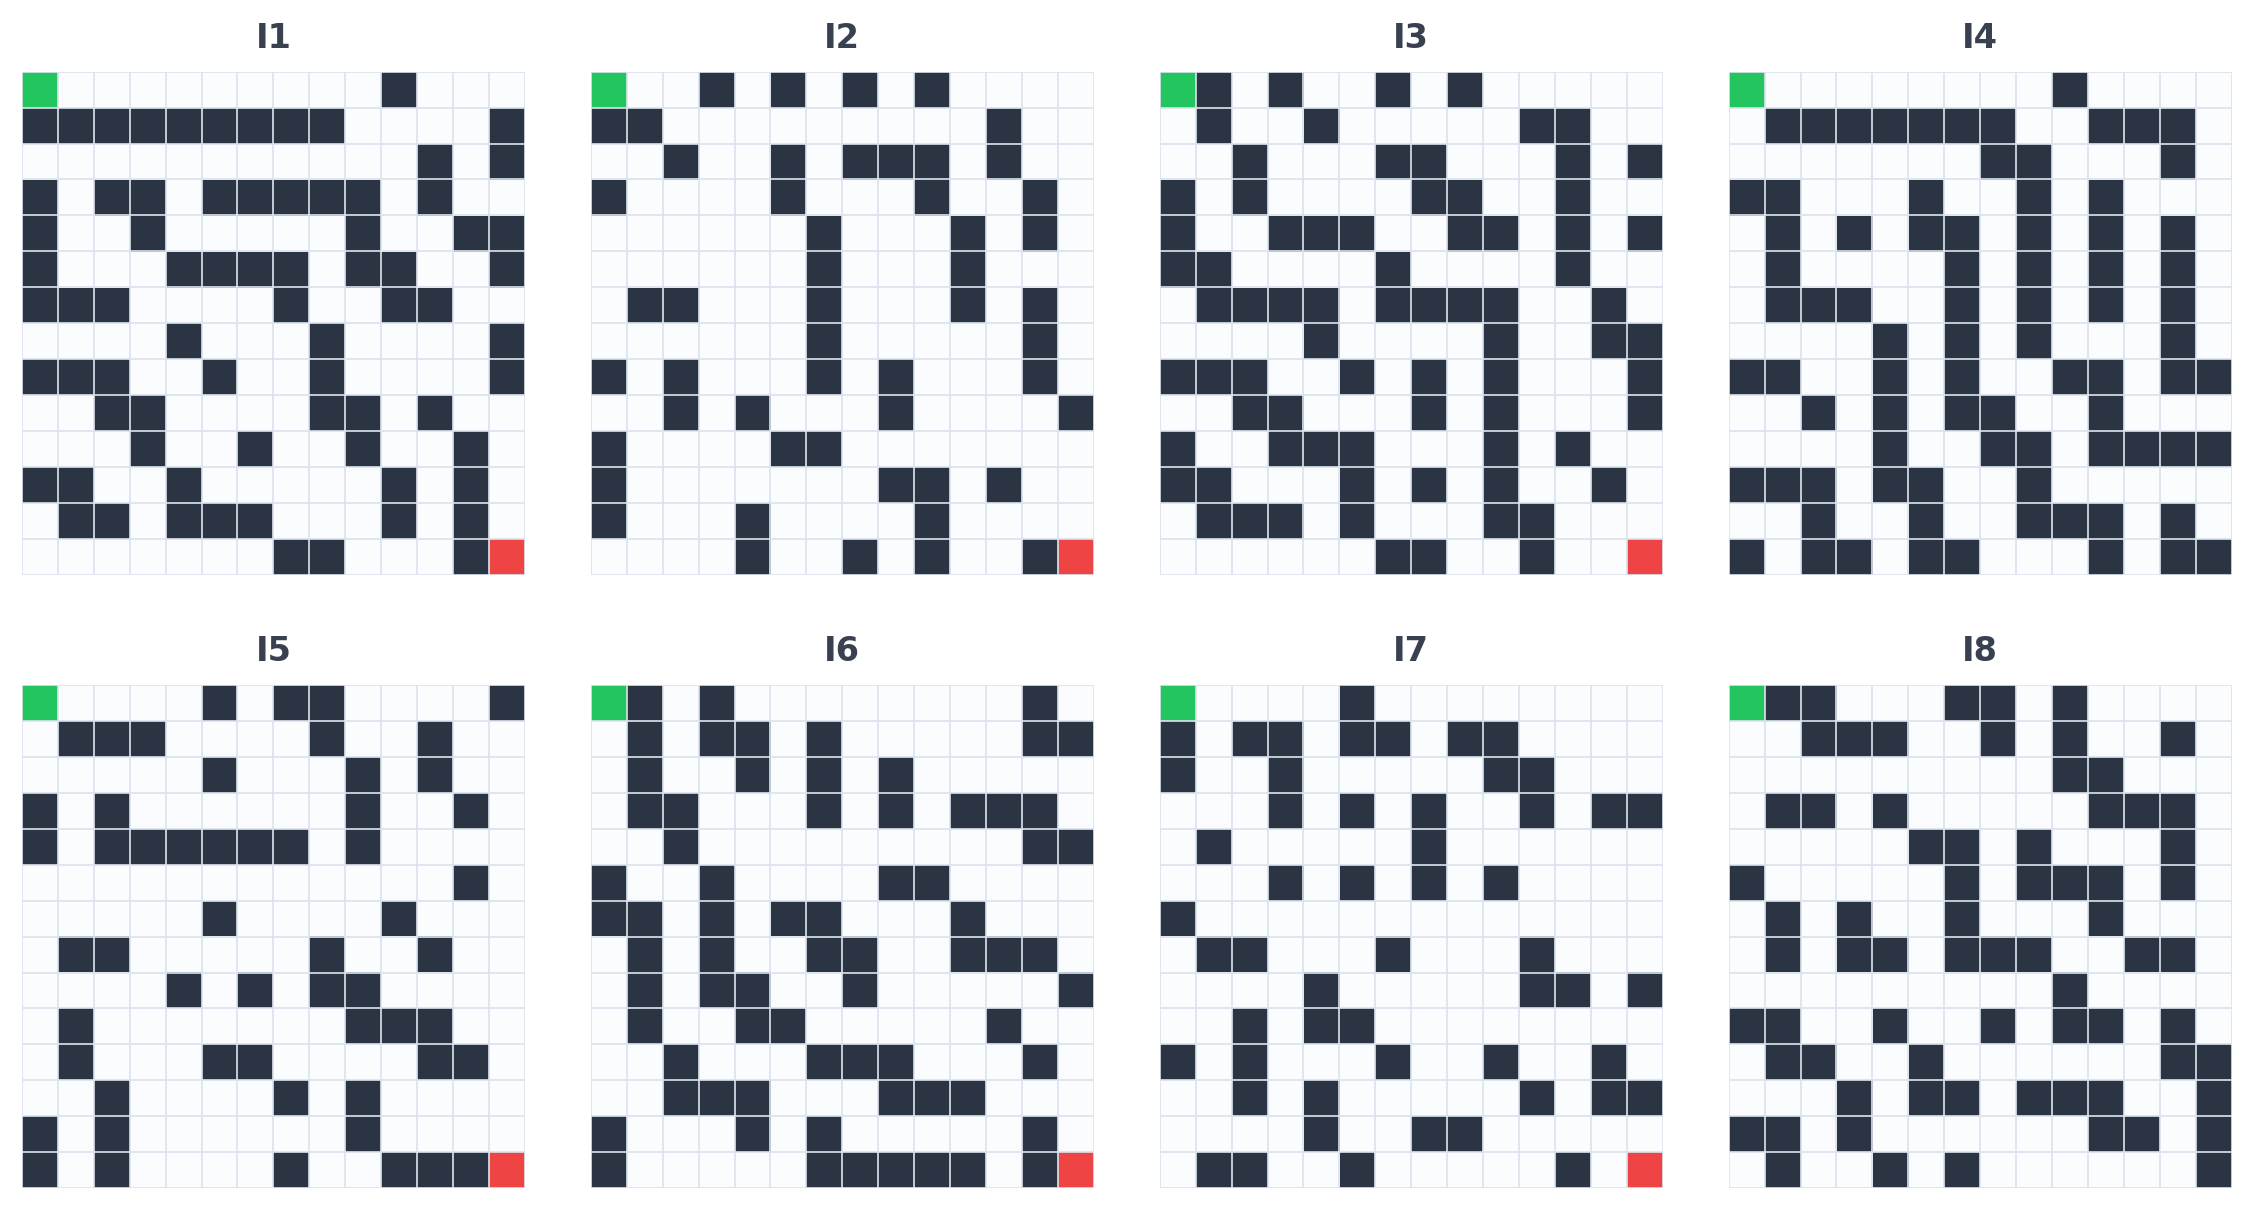
\includegraphics[width=0.92\textwidth]{figures/pcgnn/map_improved_samples.png}
    \caption{Mẫu bản đồ sinh từ genome \emph{inctyseed0.pkl}: đa dạng cấu trúc (hành lang dài, vùng mở, vật cản trung tâm) trước bước phân tầng độ khó.}
    \label{fig:pcgnn_inctyseed0_maps}
\end{figure}

Chỉ số khả năng giải trong thiết lập mê cung không áp dụng trực tiếp ở đây vì tiêu chí đó kiểm tra đường đi giữa hai góc cố định, còn đề tài yêu cầu vùng sàn liên thông đủ rộng để chiến đấu -- hai yêu cầu khác nhau. Vì vậy đề tài thay bằng \emph{reachable\_ratio} (tỷ lệ sàn liên thông).

\subsection{Nạp bản đồ vào Unity}

TilemapGenerator.cs đọc text asset theo tham số \texttt{difficulty} truyền từ ML-Agents, dựng tilemap, chạy BFS để xác nhận vùng đi được và chọn vị trí spawn. Fixed spawn (difficulty 0--2) ưu tiên ô sàn có vùng BFS rộng; random spawn (difficulty 3) lấy ngẫu nhiên từ sàn hợp lệ với \texttt{randomEnemySpawnCount}=2.

\section{Hiện thực tác nhân CombatAgent}

CombatAgent.cs kế thừa \texttt{Agent} của ML-Agents và cài đặt ba hàm chính:
\begin{itemize}
    \item \textbf{CollectObservations}: tạo vector 207D (Bảng~\ref{tab:obs_207}) bằng cách truy vấn trạng thái nhân vật, kẻ địch, đạn và 16 tia dò tường; các vị trí thiếu được điền 0.
    \item \textbf{WriteDiscreteActionMask}: tắt hành động tấn công/dash khi đang hồi, giảm mẫu lãng phí.
    \item \textbf{OnActionReceived}: giải mã 4 nhánh hành động, ghi thêm các chỉ số log tùy biến (kills/episode, clear\_rate, damage\_dealt/taken, dash\_utility, entropy) để phân tích hành vi chi tiết hơn phần thưởng đơn thuần.
\end{itemize}

\section{Cấu hình huấn luyện PPO}

Cấu hình PPO được chuẩn hóa để làm nền so sánh cho các run ablation, đặc biệt là nhóm run curriculum từ run46 trở đi. So với thiết lập thử nghiệm 200 nghìn bước trước đó, các run chính tăng lên 1--3 triệu bước do quan sát 207 chiều và bản đồ sinh theo thủ tục đòi hỏi nhiều bước huấn luyện hơn đáng kể.

\begin{table}[H]
    \centering
    \small
    \caption{Cấu hình PPO dùng trong các run chính}
    \label{tab:ppo_baseline_config}
    \begin{tabular}{|p{4cm}|c|p{7cm}|}
        \hline
        \textbf{Tham số} & \textbf{Giá trị} & \textbf{Ghi chú} \\
        \hline
        trainer\_type & ppo & Thuật toán chính. \\
        \hline
        batch\_size & 1024 & Kích thước minibatch khi cập nhật chính sách. \\
        \hline
        buffer\_size & 10240 & Số bước trải nghiệm thu thập trước mỗi lần cập nhật PPO. \\
        \hline
        learning\_rate & $3.0 \times 10^{-4}$ & Linear schedule. \\
        \hline
        beta & $5.0 \times 10^{-3}$ & Hệ số entropy bonus. \\
        \hline
        epsilon & 0.2 & PPO clipping. \\
        \hline
        lambd & 0.95 & GAE. \\
        \hline
        num\_epoch & 3 & Số epoch trên mỗi buffer. \\
        \hline
        hidden\_units & 256 & MLP actor-critic. \\
        \hline
        num\_layers & 2 & Hai lớp ẩn. \\
        \hline
        time\_horizon & 64 & Độ dài trajectory trước khi update. \\
        \hline
        max\_steps & 1M hoặc 3M & 1M cho baseline nhanh, 3M cho curriculum chính. \\
        \hline
    \end{tabular}
\end{table}

Các cấu hình phần thưởng nội tại bổ sung tín hiệu nội tại từ ICM hoặc RND. Các cấu hình LSTM thêm bộ nhớ có kích thước 256 và chuỗi quan sát dài 64 bước. Các cấu hình curriculum thêm tham số environment\_parameters.difficulty để trainer tự chuyển bài học dựa trên phần thưởng đã làm mượt.

\section{Thiết kế ablation}

Mỗi nhóm thí nghiệm loại trừ chỉ thay đổi một yếu tố chính so với cấu hình tham chiếu. Mục tiêu không phải tìm tổ hợp tối ưu tuyệt đối, mà là xác định yếu tố nào thực sự tạo cải thiện trên môi trường chiến đấu sinh theo thủ tục.

\begin{table}[H]
    \centering
    \small
    \caption{Các run ablation chính}
    \label{tab:ablation_matrix_design}
    \begin{tabular}{|p{2cm}|p{5.1cm}|c|p{5.2cm}|}
        \hline
        \textbf{Run} & \textbf{Thiết lập} & \textbf{Steps log} & \textbf{Mục đích} \\
        \hline
        run34 & PPO baseline & 1.0M & Mốc so sánh không curriculum, không phần thưởng nội tại. \\
        \hline
        run35 & PPO + ICM & 1.0M & Kiểm tra intrinsic motivation theo Pathak et al. \cite{Pathak2017}. \\
        \hline
        run36 & PPO + RND & 1.0M & Kiểm tra intrinsic motivation theo Burda et al. \cite{Burda2018}. \\
        \hline
        run42 & PPO + LSTM & 1.0M & Kiểm tra lợi ích của kiến trúc bộ nhớ \cite{Hochreiter1997}. \\
        \hline
        run46 & PPO + Curriculum & 3.0M & Thí nghiệm curriculum chính. \\
        \hline
        run47 & Curriculum + LSTM & 3.0M & Kiểm tra LSTM có bổ trợ cho curriculum hay không. \\
        \hline
        run50 & Curriculum + ICM & 3.0M & Kiểm tra ICM có phục hồi khi curriculum đóng vai trò nền tảng hay không. \\
        \hline
        run54 & 4-tier fixed-to-random & 3.0M & Kiểm tra giảm phương sai vị trí sinh đầu huấn luyện. \\
        \hline
        run55 & Curriculum + reward v2 & 3.0M & Kiểm tra thay đổi thang thưởng và tăng trọng số kết quả. \\
        \hline
    \end{tabular}
\end{table}

Mỗi run trong ma trận trên được chạy một seed và dừng khi chính sách đã hội tụ, không còn cải thiện đáng kể. Các run curriculum chính gồm run46, run47, run50, run54 và run55 đều có log đến 3.0M bước, nên Chương~4 có thể so sánh trực tiếp trên cùng thang huấn luyện. Dù vậy, các kết quả vẫn được diễn giải theo hướng thực nghiệm định hướng: so sánh cẩn trọng các xu hướng lớn, tránh khẳng định quá mức với các chênh lệch nhỏ khi chưa có nhiều seed.

Ngoài ma trận ablation chính về kỹ thuật huấn luyện, đề tài thực hiện thêm hai nhóm run mở rộng về biểu diễn quan sát.

Nhóm đầu tiên là run59 -- ablation về quan sát. Run59 không được đưa vào Bảng~\ref{tab:ablation_matrix_design} vì đây là ablation về biểu diễn quan sát, không phải ablation thuần về thuật toán huấn luyện. Khác với các run 207 chiều, run59 mở rộng vector quan sát lên 210 chiều bằng cách bổ sung ba tín hiệu đường đi: hướng bước tiếp theo theo BFS trên tilemap và khoảng cách đường đi ngắn nhất đã chuẩn hóa tới kẻ địch còn sống gần nhất. Có thể xem đây là một cấu hình \emph{path-informed}, trong đó yếu tố tìm đường được đưa vào tín hiệu học để kiểm tra giả thuyết rằng nút thắt lớn của môi trường nằm ở khả năng điều hướng trong bản đồ có tường. Vì thay đổi kích thước quan sát, run59 được huấn luyện như một run mới, không khởi tạo tiếp từ checkpoint 207 chiều của các run trước.

Nhóm thứ hai là run62, trong đó lưới chiếm chỗ cục bộ được kiểm tra ở quy mô 33.45M bước. Khác với ma trận ablation chính, run62 kết hợp nhiều thay đổi đồng thời -- quan sát mở rộng, hyperparameter điều chỉnh, curriculum 4 bậc, ICM và quy mô huấn luyện lớn hơn -- vì vậy không thể cô lập tác động của từng yếu tố riêng lẻ. Đây là thí nghiệm thăm dò mở rộng, không phải ablation đơn biến. Sau khi run59 cho thấy quan sát không gian là yếu tố đột phá, đề tài xây dựng cấu hình mở rộng: thay thế 16 chiều wall ray bằng lưới chiếm chỗ cục bộ 15$\times$15 (225 chiều). Tổng kích thước quan sát do đó nâng lên \textbf{432 chiều} (13 + 4 + 225 + 54 + 120 + 16 = 432, trong đó wall ray vẫn được giữ). Run62 kết hợp cấu hình này với curriculum 4 bậc, ICM (strength 0.001), aggressive seek luôn bật và 8 môi trường song song. Mục tiêu là kiểm tra xem quan sát lưới cục bộ có thể tiệm cận hiệu năng BFS-assisted mà không cần cài cứng cơ chế tìm đường khi số bước huấn luyện tăng lên đáng kể. Quá trình huấn luyện đạt 33.45M bước trong hai session liên tiếp. Bảng~\ref{tab:run62_ppo_config} tóm tắt các tham số khác biệt so với cấu hình baseline.

\begin{table}[H]
    \centering
    \small
    \caption{Các tham số PPO khác biệt của run62 so với baseline}
    \label{tab:run62_ppo_config}
    \begin{tabular}{|p{4cm}|c|c|p{5cm}|}
        \hline
        \textbf{Tham số} & \textbf{Baseline (run34--55)} & \textbf{run62} & \textbf{Ghi chú} \\
        \hline
        VectorObservationSize & 207 & 432 & Thêm local grid 15$\times$15 (225 chiều). \\
        \hline
        batch\_size & 1024 & 2048 & Tăng để ổn định gradient với quan sát lớn hơn. \\
        \hline
        buffer\_size & 10240 & 20480 & Tăng tương ứng với batch\_size. \\
        \hline
        learning\_rate & $3.0 \times 10^{-4}$ & $5.0 \times 10^{-5}$ & Giảm để tránh bước cập nhật quá lớn. \\
        \hline
        num\_epoch & 3 & 2 & Giảm để tránh overfitting trên buffer. \\
        \hline
        max\_steps & 1M -- 3M & 50M (target) & Chạy thực tế đến 33.45M bước. \\
        \hline
        aggressive\_seek & Tắt & Bật (giá trị 1) & Kẻ địch truy đuổi tích cực hơn; phần thưởng tiếp cận tính theo khoảng cách BFS nếu tilemap có sẵn, thay vì khoảng cách Euclid. \\
        \hline
    \end{tabular}
\end{table}

\section{Trích xuất dữ liệu}

Sau khi huấn luyện, Unity ML-Agents ghi kết quả của từng run vào các event file của TensorBoard trong thư mục Assets/results. Các event file này không thuận tiện để đưa trực tiếp vào bảng và biểu đồ, vì vậy khóa luận sử dụng script scripts/extract\_run\_metrics.py để đọc log và ghi số liệu ra các file CSV.

Script sử dụng EventAccumulator của TensorBoard để đọc các scalar như phần thưởng tích lũy, entropy chính sách, tỷ lệ dọn phòng, số kẻ địch tiêu diệt, sát thương gây ra và các chỉ số phần thưởng nội tại của ICM. Kết quả trích xuất được ghi ra hai file dữ liệu:

\begin{itemize}
    \item data/run\_metrics.csv: lưu các chỉ số tổng hợp của từng run.
    \item data/rolling\_reward\_200k.csv: lưu phần thưởng trung bình trượt với cửa sổ 200 nghìn bước tại các mốc huấn luyện.
\end{itemize}

Chương~3 chỉ mô tả quy trình trích xuất để đảm bảo khả năng tái lập. Danh sách chỉ số, ý nghĩa của từng cột và các giá trị số cụ thể được trình bày ở Chương~4, nơi các kết quả được phân tích trực tiếp.
